% questions.tex —— 2004 年·普通高等学校招生考试·辽宁卷 · 题目内容片段（无答案）
% 由 tools/generate_projects.py 依来源总账自 2004/2004_数学真题_辽宁_试题.md 生成，勿手改（改源 MD 后重跑）

\gkpart{一、选择题：本大题共 12 小题，每小题 5 分，共 60 分．在每小题给出的四个选项中，只有一项是符合题目要求的．}

\begin{question}
\gkti{1}若 $\cos\theta > 0$，$\sin 2\theta < 0$，则角 $\theta$ 的终边所在象限是\mbox{（　　）}

\begin{gkopts}(4)
\task A．第一象限
\task B．第二象限
\task C．第三象限
\task D．第四象限
\end{gkopts}

\end{question}
\begin{question}
\gkti{2}对于 $0 < a < 1$，给出下列四个不等式：① $\log_a(1 + a) < \log_a\left(1 + \dfrac{1}{a}\right)$；② $\log_a(1 + a) > \log_a\left(1 + \dfrac{1}{a}\right)$；③ $a^{1+a} < a^{1+\frac{1}{a}}$；④ $a^{1+a} > a^{1+\frac{1}{a}}$．其中成立的是\mbox{（　　）}

\begin{gkopts}(4)
\task A．①与③
\task B．①与④
\task C．②与③
\task D．②与④
\end{gkopts}

\end{question}
\begin{question}
\gkti{3}已知 $\alpha$、$\beta$ 是不同的两个平面，直线 $a \subset \alpha$，直线 $b \subset \beta$，命题 $p$：$a$ 与 $b$ 无公共点；命题 $q$：$\alpha \parallel \beta$．则 $p$ 是 $q$ 的\mbox{（　　）}

\begin{gkopts}(2)
\task A．充分而不必要的条件
\task B．必要而不充分的条件
\task C．充要条件
\task D．既不充分也不必要的条件
\end{gkopts}

\end{question}
\begin{question}
\gkti{4}设复数 $z$ 满足 $\dfrac{1-z}{1+z} = \mathrm{i}$，则 $|1+z| =$\mbox{（　　）}

\begin{gkopts}(4)
\task A．$0$
\task B．$1$
\task C．$\sqrt{2}$
\task D．$2$
\end{gkopts}

\end{question}
\begin{question}
\gkti{5}甲、乙两人独立地解同一问题，甲解决这个问题的概率是 $p_1$，乙解决这个问题的概率是 $p_2$，那么恰好有 1 人解决这个问题的概率是\mbox{（　　）}

\begin{gkopts}(2)
\task A．$p_1 p_2$
\task B．$p_1(1 - p_2) + p_2(1 - p_1)$
\task C．$1 - p_1 p_2$
\task D．$1 - (1 - p_1)(1 - p_2)$
\end{gkopts}

\end{question}
\begin{question}
\gkti{6}已知点 $A(-2, 0)$、$B(3, 0)$，动点 $P(x, y)$ 满足 $\vec{PA} \cdot \vec{PB} = x^2$，则点 $P$ 的轨迹是\mbox{（　　）}

\begin{gkopts}(4)
\task A．圆
\task B．椭圆
\task C．双曲线
\task D．抛物线
\end{gkopts}

\end{question}
\begin{question}
\gkti{7}已知函数 $f(x) = \sin\left(\pi x - \dfrac{\pi}{2}\right) - 1$，则下列命题正确的是\mbox{（　　）}

\begin{gkopts}(2)
\task A．$f(x)$ 是周期为 1 的奇函数
\task B．$f(x)$ 是周期为 2 的偶函数
\task C．$f(x)$ 是周期为 1 的非奇非偶函数
\task D．$f(x)$ 是周期为 2 的非奇非偶函数
\end{gkopts}

\end{question}
\begin{question}
\gkti{8}已知随机变量 $\xi$ 的概率分布如下：

\begin{center}
\begingroup\setlength{\tabcolsep}{4pt}
\begin{tabular}{ccccccccccc}
\toprule
$\xi$ & 1 & 2 & 3 & 4 & 5 & 6 & 7 & 8 & 9 & 10 \\
\midrule
$P$ & $\dfrac{2}{3}$ & $\dfrac{2}{3^2}$ & $\dfrac{2}{3^3}$ & $\dfrac{2}{3^4}$ & $\dfrac{2}{3^5}$ & $\dfrac{2}{3^6}$ & $\dfrac{2}{3^7}$ & $\dfrac{2}{3^8}$ & $\dfrac{2}{3^9}$ & $m$ \\
\bottomrule
\end{tabular}
\endgroup
\end{center}

则 $P(\xi = 10) =$\mbox{（　　）}

\begin{gkopts}(2)
\task A．$\dfrac{2}{3^9}$
\task B．$\dfrac{2}{3^{10}}$
\task C．$\dfrac{1}{3^9}$
\task D．$\dfrac{1}{3^{10}}$
\end{gkopts}

\end{question}
\begin{question}
\gkti{9}已知点 $F_1(-\sqrt{2}, 0)$、$F_2(\sqrt{2}, 0)$，动点 $P$ 满足 $|PF_2| - |PF_1| = 2$．当点 $P$ 的纵坐标是 $\dfrac{1}{2}$ 时，点 $P$ 到坐标原点的距离是\mbox{（　　）}

\begin{gkopts}(2)
\task A．$\dfrac{\sqrt{6}}{2}$
\task B．$\dfrac{3}{2}$
\task C．$\sqrt{3}$
\task D．$2$
\end{gkopts}

\end{question}
\begin{question}
\gkti{10}设 $A$、$B$、$C$、$D$ 是球面上的四个点，且在同一平面内，$AB = BC = CD = DA = 3$，球心到该平面的距离是球半径的一半，则球的体积是\mbox{（　　）}

\begin{gkopts}(4)
\task A．$8\sqrt{6}\pi$
\task B．$64\sqrt{6}\pi$
\task C．$24\sqrt{2}\pi$
\task D．$72\sqrt{2}\pi$
\end{gkopts}

\Needspace{0.4\textheight}
\end{question}
\begin{question}
\gkti{11}若函数 $f(x) = \sin(\omega x + \varphi)$ 的图象（部分）如图所示，则 $\omega$ 和 $\varphi$ 的取值是\mbox{（　　）}
\nopagebreak[4]
\begin{center}% Candidate source: src-2323f00197bbd8d5c8353a847fc0e7ccfc52169ca219272ee58990ae4b6ecba3
% Source PDF SHA-256: be2accb36a086126db90ee7c5a217e08e55429053a4167df1ad58bbfb213de46
% PDF page 1 (printed page 180), question 11.
% Redraw follows visible wave relations; schematic curve, not a scale claim.
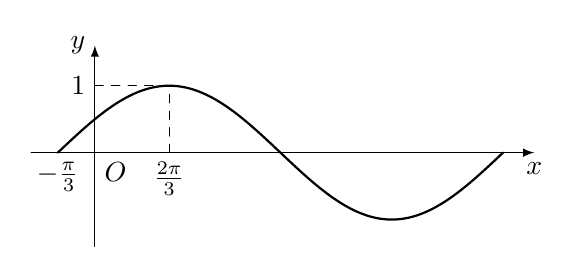
\begin{tikzpicture}[line cap=round,line join=round,>=latex,x=0.45cm,y=0.85cm]
  % Axes
  \draw[->] (-1.8,0) -- (12.4,0) node[below] {$x$};
  \draw[->] (0,-1.4) -- (0,1.6) node[left] {$y$};
  \node[below right] at (0,0) {$O$};

  % Function: f(x) = sin(0.5*x + pi/6), full period from -pi/3 to 11pi/3 landing on x-axis
  \draw[thick, smooth, domain={-3.1415926/3}:{11*3.1415926/3}, samples=100] plot (\x, {sin((0.5*\x + 3.1415926/6) r)});

  % Dashed projections for peak at (2pi/3, 1)
  \draw[dashed] ({2*3.1415926/3}, 0) -- ({2*3.1415926/3}, 1);
  \draw[dashed] (0, 1) -- ({2*3.1415926/3}, 1);

  % Ticks and labels
  \node[below] at ({-3.1415926/3}, 0) {$-\frac{\pi}{3}$};
  \node[below] at ({2*3.1415926/3}, 0) {$\frac{2\pi}{3}$};
  \node[left] at (0, 1) {$1$};
\end{tikzpicture}
\end{center}
\nopagebreak[4]
\begin{gkopts}(1)
\task A．$\omega = 1, \varphi = \dfrac{\pi}{3}$
\task B．$\omega = 1, \varphi = -\dfrac{\pi}{3}$
\task C．$\omega = \dfrac{1}{2}, \varphi = \dfrac{\pi}{6}$
\task D．$\omega = \dfrac{1}{2}, \varphi = -\dfrac{\pi}{6}$
\end{gkopts}

\end{question}
\begin{question}
\gkti{12}有两排座位，前排 11 个座位，后排 12 个座位，现安排 2 人就座，规定前排中间的 3 个座位不能坐，并且这 2 人不左右相邻，那么不同排法的种数是\mbox{（　　）}

\begin{gkopts}(4)
\task A．$234$
\task B．$346$
\task C．$350$
\task D．$363$
\end{gkopts}

\end{question}
\gkpart{二、填空题：本大题共 4 小题，每小题 4 分，共 16 分．把答案填在题中横线上．}

\begin{question}
\gkti{13}若经过点 $P(-1, 0)$ 的直线与圆 $x^2 + y^2 + 4x - 2y + 3 = 0$ 相切，则此直线在 $y$ 轴上的截距是 \underline{\hspace{3cm}}．

\end{question}
\begin{question}
\gkti{14}$\lim_{x \to \pi} \dfrac{(x - \pi)\cos x}{\sqrt{x} - \sqrt{\pi}} =$ \underline{\hspace{3cm}}．

\Needspace{0.4\textheight}
\end{question}
\begin{question}
\gkti{15}如图，四棱柱 $ABCD - A_1B_1C_1D_1$ 的底面 $ABCD$ 为正方形，侧棱与底面边长均为 $2a$，且 $\angle A_1AD = \angle A_1AB = 60^\circ$，则侧棱 $AA_1$ 和截面 $B_1D_1DB$ 的距离是 \underline{\hspace{3cm}}．
\nopagebreak[4]
\begin{center}% Candidate source: src-2323f00197bbd8d5c8353a847fc0e7ccfc52169ca219272ee58990ae4b6ecba3
% Source PDF SHA-256: be2accb36a086126db90ee7c5a217e08e55429053a4167df1ad58bbfb213de46
% PDF page 1 (printed page 180), question 15.
% Redraw follows visible/hidden edges; oblique quadrangular prism ABCD-A1B1C1D1.
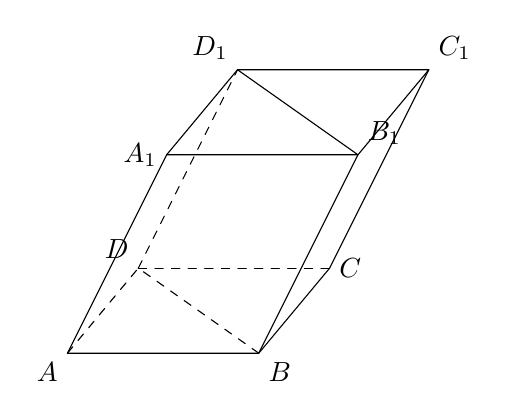
\begin{tikzpicture}[line cap=round,line join=round,>=latex,x=0.9cm,y=0.9cm]
  % Base vertices
  \coordinate (A) at (-1.5,-1.2);
  \coordinate (B) at (1.2,-1.2);
  \coordinate (C) at (2.2,0);
  \coordinate (D) at (-0.5,0);

  % Top vertices shifted by (1.4, 2.8)
  \coordinate (A1) at (-0.1,1.6);
  \coordinate (B1) at (2.6,1.6);
  \coordinate (C1) at (3.6,2.8);
  \coordinate (D1) at (0.9,2.8);

  % Hidden edges
  \draw[dashed] (A) -- (D);
  \draw[dashed] (D) -- (C);
  \draw[dashed] (D) -- (D1);
  \draw[dashed] (B) -- (D);

  % Visible edges: base
  \draw (A) -- (B) -- (C);

  % Visible edges: lateral
  \draw (A) -- (A1);
  \draw (B) -- (B1);
  \draw (C) -- (C1);

  % Visible edges: top
  \draw (A1) -- (B1) -- (C1) -- (D1) -- cycle;

  % Diagonal on top face
  \draw (B1) -- (D1);

  % Labels
  \node[below left] at (A) {$A$};
  \node[below right] at (B) {$B$};
  \node[right] at (C) {$C$};
  \node[above left] at (D) {$D$};
  \node[left] at (A1) {$A_1$};
  \node[above right] at (B1) {$B_1$};
  \node[above right] at (C1) {$C_1$};
  \node[above left] at (D1) {$D_1$};
\end{tikzpicture}
\end{center}
\nopagebreak[4]
\end{question}
\begin{question}
\gkti{16}口袋内装有 10 个相同的球，其中 5 个球标有数字 0，5 个球标有数字 1，若从袋中摸出 5 个球，那么摸出的 5 个球所标数字之和小于 2 或大于 3 的概率是 \underline{\hspace{3cm}}．（以数值作答）

\end{question}
\gkpart{三、解答题：本大题共 6 小题，共 74 分．解答应写出文字说明、证明过程或演算步骤．}

\Needspace{0.4\textheight}
\begin{question}
\gkti{17}（本小题满分 12 分）

已知四棱锥 $P - ABCD$，底面 $ABCD$ 是菱形，$\angle DAB = 60^\circ$，$PD \perp$ 平面 $ABCD$，$PD = AD$，点 $E$ 为 $AB$ 中点，点 $F$ 为 $PD$ 中点．

（1）证明：平面 $PED \perp$ 平面 $PAB$；

（2）求二面角 $P - AB - F$ 的平面角的余弦值．
\nopagebreak[4]
\begin{center}% Candidate source: src-2323f00197bbd8d5c8353a847fc0e7ccfc52169ca219272ee58990ae4b6ecba3
% Source PDF SHA-256: be2accb36a086126db90ee7c5a217e08e55429053a4167df1ad58bbfb213de46
% PDF page 1 (printed page 180), question 17.
% Redraw follows visible/hidden edges; quadrangular pyramid P-ABCD with rhombus base.
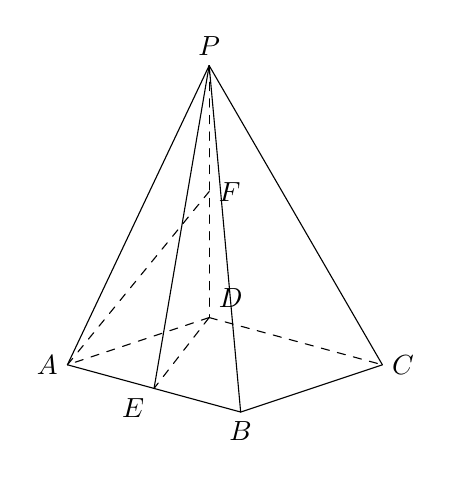
\begin{tikzpicture}[line cap=round,line join=round,>=latex,x=1.0cm,y=1.0cm]
  % Vertices
  \coordinate (D) at (0,0);
  \coordinate (P) at (0,3.2);
  \coordinate (A) at (-1.8,-0.6);
  \coordinate (C) at (2.2,-0.6);
  \coordinate (B) at (0.4,-1.2);

  % Midpoints E on AB and F on PD
  \coordinate (E) at (-0.7,-0.9);
  \coordinate (F) at (0,1.6);

  % Hidden edges
  \draw[dashed] (P) -- (D);
  \draw[dashed] (D) -- (A);
  \draw[dashed] (D) -- (C);
  \draw[dashed] (D) -- (E);
  \draw[dashed] (A) -- (F);

  % Visible edges: lateral
  \draw (P) -- (A);
  \draw (P) -- (B);
  \draw (P) -- (C);
  \draw (P) -- (E);

  % Visible edges: base
  \draw (A) -- (B) -- (C);

  % Labels
  \node[above] at (P) {$P$};
  \node[right] at (F) {$F$};
  \node[above right] at (D) {$D$};
  \node[left] at (A) {$A$};
  \node[below left] at (E) {$E$};
  \node[below] at (B) {$B$};
  \node[right] at (C) {$C$};
\end{tikzpicture}
\end{center}
\nopagebreak[4]
\end{question}
\begin{question}
\gkti{18}（本小题满分 12 分）

设全集 $U = \mathbf{R}$．

（1）解关于 $x$ 的不等式 $|x - 1| + a - 1 > 0$（$a \in \mathbf{R}$）；

（2）记 $A$ 为（1）中不等式的解集，集合 $B = \left\{x \;\middle|\; \sin\left(\pi x - \dfrac{\pi}{3}\right) + \sqrt{3}\cos\left(\pi x - \dfrac{\pi}{3}\right) = 0\right\}$，若 $(\complement_U A) \cap B$ 恰有 3 个元素，求 $a$ 的取值范围．

\end{question}
\begin{question}
\gkti{19}（本小题满分 12 分）

设椭圆方程为 $x^2 + \dfrac{y^2}{4} = 1$，过点 $M(0, 1)$ 的直线 $l$ 交椭圆于点 $A$、$B$，$O$ 是坐标原点，点 $P$ 满足 $\vec{OP} = \dfrac{1}{2}(\vec{OA} + \vec{OB})$，点 $N$ 的坐标为 $\left(\dfrac{1}{2}, \dfrac{1}{2}\right)$，当 $l$ 绕点 $M$ 旋转时，求：

（1）动点 $P$ 的轨迹方程；

（2）$|\vec{NP}|$ 的最小值与最大值．

\end{question}
\begin{question}
\gkti{20}（本小题满分 12 分）

甲方是一农场，乙方是一工厂．由于乙方生产须占用甲方的资源，因此甲方有权向乙方索赔以弥补经济损失并获得一定净收入，在乙方不赔付甲方的情况下，乙方的年利润 $x$（元）与年产量 $t$（吨）满足函数关系 $x = 2000\sqrt{t}$．若乙方每生产一吨产品必须赔付甲方 $s$ 元（以下称 $s$ 为赔付价格）．

（1）将乙方的年利润 $w$（元）表示为年产量 $t$（吨）的函数，并求出乙方获得最大利润的年产量；

（2）甲方每年受乙方生产影响的经济损失金额 $y = 0.002t^2$（元），在乙方按照获得最大利润的产量进行生产的前提下，甲方要在索赔中获得最大净收入，应向乙方要求的赔付价格 $s$ 是多少？

\end{question}
\begin{question}
\gkti{21}（本小题满分 12 分）

已知函数 $f(x) = ax - \dfrac{3}{2}x^2$ 的最大值不大于 $\dfrac{1}{6}$，又当 $x \in \left[\dfrac{1}{4}, \dfrac{1}{2}\right]$ 时，$f(x) \geqslant \dfrac{1}{8}$．

（1）求 $a$ 的值；

（2）设 $0 < a_1 < \dfrac{1}{2}$，$a_{n+1} = f(a_n)$，$n \in \mathbf{N}^*$．证明 $a_n < \dfrac{1}{n+1}$．

\end{question}
\begin{question}
\gkti{22}（本小题满分 14 分）

已知函数 $f(x) = \ln(\mathrm{e}^x + a)$（$a > 0$）．

（1）求函数 $y = f(x)$ 的反函数 $y = f^{-1}(x)$ 及 $f(x)$ 的导数 $f'(x)$；

（2）假设对任意 $x \in [\ln(3a), \ln(4a)]$，不等式 $|m - f^{-1}(x)| + \ln(f'(x)) < 0$ 成立，求实数 $m$ 的取值范围．

\end{question}